%\documentclass[a4paper,12pt,final]{article}
% Pour une impression recto verso, utilisez plutôt ce documentclass :
\documentclass[a4paper,12pt,twoside,final]{article}

\usepackage[english,francais]{babel}
\usepackage[utf8]{inputenc}
\usepackage[T1]{fontenc}
\usepackage[pdftex]{graphicx}
\usepackage{setspace}
\usepackage{xcolor}
\usepackage[hidelinks]{hyperref}
\usepackage[french]{varioref}
\usepackage{algorithm}
\usepackage{algorithmic}
\usepackage{qtree}
\usepackage{array}
\usepackage{multirow}

\newcommand\rmq[2][green!50!black]{\marginpar{\hspace*{-0.5em}\begin{minipage}{0.25\textwidth}\scriptsize\if\empty#1\empty\else\color{#1}\fi
      #2
    \end{minipage}
  }}
\newcommand\rmqinline[1]{{\footnotesize \color{green!50!black} #1}}

\newcommand{\reporttitle}{Algorithme de recherche dans des données de séquençage ADN avec la transformée de Burrows-Wheeler à contexte borné}     % Titre
\newcommand{\reportauthor}{Marion \textsc{Tommasi}} % Auteur
\newcommand{\reportsubject}{Stage de Licence 3 informatique} % Sujet
\newcommand{\HRule}{\rule{\linewidth}{0.5mm}}
\setlength{\parskip}{1ex} % Espace entre les paragraphes
%\renewcommand{\baselinestretch}{1.5}

\newcommand{\adn}{\textsc{adn\xspace}}
\newcommand{\bwt}{\textsc{bwt\xspace}}
\newcommand{\kbwt}{$k$-\textsc{bwt\xspace}}

\hypersetup{
    pdftitle={\reporttitle},%
    pdfauthor={\reportauthor},%
    pdfsubject={\reportsubject},%
    pdfkeywords={rapport} {L3} {bio-informatique} {algorithmique du texte}
}

\begin{document}
  % Inspiré de http://en.wikibooks.org/wiki/LaTeX/Title_Creation

\begin{titlepage}

\begin{center}

\begin{minipage}[t]{0.48\textwidth}
  \begin{flushleft}
%    
\includegraphics [width=30mm]{images/logo-univ.png} \\[0.5cm]
    \begin{spacing}{1.5}
      \textsc{\large Université de Lille 1}
    \end{spacing}
  \end{flushleft}
\end{minipage}
%{
\includegraphics [width=30mm]{images/INRIA_logo.png} \\[0.5cm]}
\begin{minipage}[t]{0.48\textwidth}
  \begin{flushright}
%    
\includegraphics [width=30mm]{images/INRIA_logo.png} \\[0.5cm]
    \textsc{\large Équipe Bonsai}
  \end{flushright}
\end{minipage} \\[1.5cm]

%\begin{minipage}[t]{0.48\textwidth}
%    
\includegraphics [width=30mm]{images/logo-univ.png} \\[0.5cm]
%    
\includegraphics [width=30mm]{images/INRIA_logo.png} \\[0.5cm]
%\end{minipage}
%
%\begin{minipage}[t]{0.48\textwidth}
%  \begin{flushright}
%	\textsc{\large Université de Lille 1}
%  \end{flushright}
%  \begin{flushleft}
%    \textsc{\large Équipe Bonsai}
%  \end{flushleft}
%\end{minipage}


\textsc{\Large \reportsubject}\\[0.5cm]
\HRule \\[0.4cm]
{\LARGE \bfseries \reporttitle}\\[0.4cm]
\HRule \\[1.5cm]

\begin{minipage}[t]{0.3\textwidth}
  \begin{flushleft} \large
    \emph{Auteur :}\\
    \reportauthor
  \end{flushleft}
\end{minipage}
\begin{minipage}[t]{0.6\textwidth}
  \begin{flushright} \large
    \emph{Responsables :} \\
    Rayan \textsc{Chikhi} \\
    Mikael \textsc{Salson}
  \end{flushright}
\end{minipage}

\vfill

{\large 30 mars - 30 juin 2015}

\end{center}

\end{titlepage}

  \cleardoublepage % Dans le cas du recto verso, ajoute une page blanche si besoin
  \tableofcontents % Table des matières
  \sloppy          % Justification moins stricte : des mots ne dépasseront pas des paragraphes
  \cleardoublepage
  \section*{Remerciements}
\addcontentsline{toc}{section}{Remerciements}

Je tiens à remercier toutes les personnes qui m'ont aidées pendant ce stage et à la rédaction de ce rapport.

En particulier, je voudrais remercier mes maîtres de stage Rayan Chikhi et Mikael Salson pour m'avoir aidée et guidée tout au long de ce stage, ainsi que toute l'équipe Bonsai pour m'avoir chaleureusement accueillie en son sein.

Je voudrais aussi remercier mes amis et ma famille qui m'ont aidé pour la rédaction de ce rapport.


%\footnotetext{
%http://www.ukonline.be/programmation/latex/tutoriel/index.php et \\
%http://blog.hikoweb.net/index.php?/post2011/11/06/Exemple-de-rapport-en-LaTeX}


%\uparrow\cite{tutoltx}\cite{expltx}}

%Voici une note\,\footnote{Texte de bas de page} de bas de page.
%Une deuxième\,\footnotemark{} déclarée différemment.
%La même note\,\footnotemark[\value{footnote}].
%
%\footnotetext{Il a deux références vers cette note}
  \cleardoublepage
  \section*{Introduction} % Pas de numérotation
\addcontentsline{toc}{section}{Introduction} % Ajout dans la table des matières

Le séquençage de l'ADN est depuis plus de 20 ans un sujet important de la bio-informatique, avec de applications aussi bien en biologie fondamentale qu'en médecine. Qu'il serve à étudier l'évolution ou des maladies, la demande est de lus en plus importante.

De plus, depuis l'émergence des techniques de séquençage haut débit, la masse de données biologiques a augmenté plus vite que les algorithmes existants ne sont capables de les traiter. Le besoin d'améliorer ces algorithmes est donc de plus en plus pressant, à chaque étape du traitement et de l'analyse de ces données.

La compression et l'indexation des reads, fragments d'ADN retournés par les séquenceurs, est notamment un sujet sur lequel peu de recherches ont été menées, malgré la taille grandissante de ces données.

Néanmoins, beaucoup d'algorithme sur la compression de données existent déjà, et sont utilisés pour stocker l'ADN.

Le travail présenté ici porte donc sur l'étude de l'un de ces algorithmes, \textit{la transformée de Burrows-Wheeler à contexte borné}, et son amélioration pour ce type de données particuliers que sont les reads.

Ce travail a été réalisé au cours du stage de fin de licence informatique à Lille 1, dans l'équipe de bio-informatique Bonsai.

%Dans le cadre de ma troisième année de licence informatique, j'ai effectué un stage de recherche à l'Inria. Du 30 mars au 30 juin, dans l'équipe Bonsai, j'ai travaillé sur l'algorithmique du texte appliquée à la bio-informatique.

%Ce stage a été pour moi l'opportunité d'approfondir mes connaissances sur la bio-informatique, ainsi que sur diverses structures de données telles que les arbres ou les tableaux de suffixes. Il m'a également permis de découvrir le monde de la recherche et de participer à des conférences.

%Mon travail a consisté essentiellement en l'étude, l'amélioration et l'implémentation d'un algorithme de compression et d'indexation de texte.


%Afin de rendre de compte de ce stage, il parait important de présenter l'équipe dans lequel il s'est déroulé, ainsi que le champ de recherche sur lequel il portait. Il apparaît ensuite nécessaire d'expliquer l'état de l'art concernant le problème posé par le sujet de stage. On pourra alors exposer le travail réaliser pendant ce stage, en revenant d'abord sur le sujet, puis en expliquant les pistes suivies, pour enfin s'intéresser aux résultats.
  \section{Contexte}

%
%\subsection{L'équipe}
%
%Mon stage s'est déroulé au sein de l'équipe Bonsai, équipe de recherche affiliée à l'Inria Lille - Nord Europe et le Centre de Recherche en Informatique, Signal et Automatique de Lille (CRIStAL, Université Lille 1, CNRS). 
%
%\subsubsection{Bonsai}
%L'équipe Bonsai compte 20 personnes, dont 10 membres permanents, sous la responsabilité d'Hélène Touzet. Le principal objectif de l'équipe est de développer des algorithmes d'analyse de séquences biologiques, que ce soit pour l'étude de l'ADN, de l'ARN, des protéines ou des NRP (peptides non-ribosomiques). Ce travail se réalise souvent en collaborations avec des biologistes, et se concrétise par la création de logiciels. Vidgil, par exemple, est une plate-forme  d'analyse des données de séquençage haut débit développée par l'équipe et utilisée à l'institut Pasteur pour suivre l'évolution de leucémies.
%


\subsection{Séquençage}
Le séquençage consiste à déterminer l'ordre des composants de molécules. Le séquençage de l'ADN sert à déterminer l'ordre des nucléotides composant un fragment donné. Pour cela, diverses techniques existent. Historiquement, la méthode la plus utilisée a été celle dite de Sanger, d'après son inventeur, plus facile à robotiser que celle de Maxam et Gilbert, développée à la même époque. Cependant, depuis quelques années, de nouvelles méthodes plus efficaces de séquençage haut débit sont apparues, multipliant le nombre de données issues du séquençage.

\subsubsection{Méthode de Sanger}
L'ADN polymérase est une enzyme utilisée dans la réplication de l'ADN, qui permet de créer des molécules d'ADN en assemblant des nucléotides. Les nucléotides utilisés lors de la réplication sont des désoxyribonucléotides (dNTP), mais il existe aussi des didésoxyribonucléotides (ddNTP), qui forcent l’arrêt de la réaction à la suite de leur utilisation. 

La méthode de Sanger consiste à répliquer un brin d'ADN dans un milieu où se trouvent des dNTP ainsi que de quelques ddNTP d'un seul type (ddNTP à Guanine, Thymine, Adénine ou Cytosine\rmq{définis-les avant}). La réplication va donc s’arrêter aléatoirement sur l'un des nucléotides correspondant à la ddNTP choisie. Cette expérience est répétée quatre fois, avec les quatre types de ddNTP, puis l'on compare les longueurs des brins d'ADN répliqués par chromatographie.


\begin{figure}[!ht]
    \center
    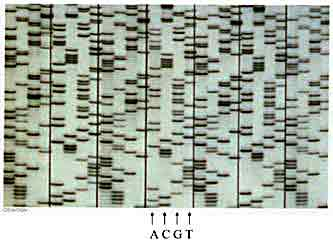
\includegraphics[]{./images/chromato_acanthoweb.jpg}
    \rmqinline{Précise la source}
    \caption{Exemple de chromatographie}
    \label{chromato}
\end{figure}


Il ne reste plus qu'à lire la séquence ADN, processus automatisable mais long.

\subsubsection{Séquençage haut débit}
Il existe de nombreuses techniques de séquençage haut débit, plus ou moins chères, fiables ou efficaces.
Par exemple, le séquençage par synthèse, utilisé par l'entreprise \emph{Illumina}, est basé sur l'utilisation de colorants fluorescents.

Pour cette méthode, on attache aux séquences étudiées des amorces, qui servent à la synthèse de l'ADN. Puis avec l'ajout de nucléotides et d'ADN polymérase, ces séquences sont amplifiées. On ajoute enfin des nucléotides associés à des couleurs spécifiant leur type (Guanine, Thymine, Cytosine et Adénine), qui vont s'associer à leur complémentaire sur les brins d'ADN. Les nucléotides non-attachés sont ensuite enlevés, et les colorants excités et photographiés. Les colorants sont retirés chimiquement et le processus répété plusieurs fois jusqu'à ce que l'ensemble de l'ADN soit séquencé.

\subsubsection{Reads}
Les données retournées par les séquenceurs sont appelées des \emph{reads}. Ce sont de très nombreux fragments de l'ADN séquencé. La taille et le nombre de ces fragments varient, mais ils sont souvent composés de 100 à 300 nucléotides et couvrent au moins 30 à 40 fois la séquence initiale. 

Ce sont donc des données très redondantes, ce que nous chercherons à exploiter dans ce stage.


\subsection{Structures de données utilisées}
La suite de ce rapport se concentrera sur une façon de compresser et indexer les reads. Pour cela, nous allons utiliser plusieurs structures de données, notamment des tableaux de suffixes et des wavelet tree que nous présentons ici.

\subsubsection{Tableau de suffixes}
Un suffixe d'une chaîne de caractères $s$ est une chaîne $s'$ plus petite telle que $s'$ termine $s$. C'est-à-dire tel qu'il existe une chaîne $p$, pouvant être vide, telle que $p + s' = s$, ($+$ représentant la concaténation des chaînes). $p$ est d'ailleurs un préfixe de $s$.

Un tableau de suffixes est un tableau d'entiers représentant tous les suffixes d'une chaîne. Pour le construire, il faut construire l'ensemble des suffixes, en attribuant à chaque suffixe un entier présentant son ordre dans le texte. Les suffixes sont ensuite triés par ordre lexicographique, et seule leur place est gardée. La figure \ref{suffixes} illustre cette construction.

\begin{figure}[h!]
\fbox{%
  \begin{minipage}{0.4\linewidth}
  	\begin{flushleft}
      \textsc{%
  	  \begin{tabular}{l|c|}
  	  	suffixe & indice \tabularnewline \hline
        barbapapa\$ & 0\\
	    arbapapa\$ & 1\\
	    rbapapa\$ & 2\\
	    bapapa\$ & 3\\
	    apapa\$ & 4\\
	    papa\$ & 5\\
	    apa\$ & 6\\
	    pa\$ & 7\\
        a\$ & 8\\
	    \$ & 9
	  \end{tabular} 
	  }
  	\end{flushleft}
  \end{minipage}%
  \begin{minipage}{0.2\linewidth}
	\begin{center}
		tri\\
  		$\rightarrow$
	\end{center}
  \end{minipage}%
  \begin{minipage}{0.4\linewidth}
  	\begin{flushright}
      \textsc{%
  	  \begin{tabular}{|l|c}
  	  	suffixe & indice\tabularnewline \hline
	    \$ & {\color{red}9}\\
        a\$ & {\color{red}8}\\
	    apa\$ & {\color{red}6}\\
	    apapa\$ & {\color{red}4}\\
	    arbapapa\$ & {\color{red}1}\\
	    bapapa\$ & {\color{red}3}\\
	    barbapapa\$ & {\color{red}0}\\
	    pa\$ & {\color{red}7}\\
        papa\$ & {\color{red}5}\\
	    rbapapa\$ & {\color{red}2}\\
	  \end{tabular} 
	  }
  	\end{flushright}
  \end{minipage}%
}
\caption{Construction du tableau des suffixes (en rouge) pour la chaîne "\textsc{barbapapa\$}"}
\label{suffixes}
\end{figure}

\subsubsection{Wavelet tree}
Les arbres sont des structures de données couramment utilisées en informatique, représentant des graphes acycliques orientés, tels que tous les nœuds sauf un, la racine, ont un unique parent. Pour les arbres binaires, comme le wavelet tree, les nœuds ont au plus deux fils. Les nœuds n'ayant pas de fils sont appelés feuilles.

Le \textit{wavelet tree}, ou arbre d'ondelettes, est une structure de données succincte (c'est-à-dire compressée presque\rmq{stockée optimalement, plutôt} optimalement), à l'origine utilisée pour représenter les tableaux de suffixes compressés.

La construction du wavelet tree est basée sur la division de l'alphabet du mot d'origine en deux. Cette division peut se faire par ordre lexicographique, ou par d'autres algorithmes plus complexes tels que le codage de Huffman. Nous ne nous intéresserons ici qu'à la première façon.

Prenons comme exemple la construction du wavelet tree de \textsc{"barbapapa\$"}. L'alphabet est l'ensemble \textsc{\{'\$'; 'a'; 'b'; 'p'; 'r'\}}. Les lettres appartenant à la première moitié de l'alphabet (\textsc{\{'\$'; 'a'\}}) seront représentées par un 0, tandis que les lettres de la deuxième moitié seront des 1. La racine comporte donc le mot "1011010100".

Les deux moitiés de l'alphabet descendent dans les fils de la racine. Le premier nœud code donc \textsc{"aaaa\$} sur l'alphabet \textsc{\{'\$'; 'a'\}}, et le deuxième nœud code \textsc{"brbpp"} sur l'alphabet \textsc{\{'b'; 'r'; 'p'\}}. La même opération que sur la racine est alors renouvelée, jusqu'à ce que les nœuds ne codent plus qu'une seule lettre.

%Exemple

\subsection{Transformée de Burrows-Wheeler}

La transformée de Burrows-Wheeler\up{\cite{bwt}}, abrégée \bwt, est un algorithme de réorganisation des données, fréquemment utilisé pour compresser les données. C'est un algorithme réversible qui augmente la probabilité que des caractères identiques se retrouvent à côté. Il\rmq{Il ?} est notamment utilisé dans l'algorithme de compression \emph{bzip2}.

\subsubsection{Construction}
La construction de la \bwt\ est simple : elle consiste à prendre la dernière lettre de toutes les rotations de la chaîne initiale triées lexicographiquement.
Une rotation de $k$ éléments d'une chaîne de caractères de longueur $n$ est composée des $n-k$ derniers éléments de la chaîne concaténés aux $k$ premiers.
Ainsi, on peut voir l'ensemble des rotations d'une chaîne de caractères "\textsc{barbapapa\$}" dans la figure \ref{rotations}.

\begin{figure}[h!]
\fbox{%
  \begin{minipage}{\linewidth}
  	\begin{center}
 \textsc{%
      barbapapa\$\\
	  arbapapa\$b\\
	  rbapapa\$ba\\
	  bapapa\$bar\\
	  apapa\$barb\\
	  papa\$barba\\
	  apa\$barbap\\
	  pa\$barbapa\\
      a\$barbapap\\
	  \$barbapapa
	  }
	\end{center}
  \end{minipage}%
}
\caption{Ensemble des rotations de la chaîne "\textsc{barbapapa\$}"}
\label{rotations}
\end{figure}

Ordonnés par ordre lexicographique, on obtient l'exemple \ref{bwt}, où l'on ne garde que la dernière lettre pour avoir la \bwt.
\begin{figure}[h!]
\fbox{%
  \begin{minipage}{\linewidth}
    t = "\textsc{barbapapa\$}"
  	\begin{center}
  	  \textsc{%
      \$barbapap {\color{red}a}\\
      a\$barbapa {\color{red}p}\\
	  apa\$barba {\color{red}p}\\
	  apapa\$bar {\color{red}b}\\
	  arbapapa\$ {\color{red}b}\\
	  bapapa\$ba {\color{red}r}\\
	  barbapapa {\color{red}\$}\\
	  pa\$barbap {\color{red}a}\\
	  papa\$barb {\color{red}a}\\
	  rbapapa\$b {\color{red}a}
	  }
	\end{center}
	\bwt(t) = "\textsc{appbbr\$aaa}"
  \end{minipage}%
}
\caption{Construction de la \bwt\ de "\textsc{barbapapa\$}"}
\label{bwt}
\end{figure}

On peut d'ailleurs remarquer dans la \bwt\ les suites consécutives de P, B et A. En effet, lorsque les lettres sont suivies des mêmes caractères, elles vont se retrouver à côté dans la \bwt, facilitant ainsi la compression.

\subsubsection{Réversibilité}
Lorsqu'un algorithme est réversible, c'est que l'on peut retrouver sa donnée de départ à partir de son résultat. C'est donc une propriété importante de la \bwt, puisqu'elle permet de retrouver le texte de départ.\rmq{Tu peux faire le lien avec la décompression}

Pour assurer la réversibilité de la \bwt, on ajoute un caractère spécial, lexicographiquement plus petit que tous les autres et traditionnellement représenté par \$. Ainsi, on est assuré de savoir où se termine la chaîne initiale.

Pour inverser la \bwt, on reconstruit le tableau des rotations, colonne par colonne.
Tout d'abord, la dernière colonne correspond à la \bwt, et la première à l'ensemble des lettres dans l'ordre lexicographique. Comme ce sont des rotations, les lettres de la première colonne suivent celles de la dernière \rmq{dans le texte d'origine}. En triant ces groupes de deux lettres, on obtient donc la deuxième colonne, comme dans la figure \ref{unbwt}

\begin{figure}[h!]
\fbox{%
  \begin{minipage}{\linewidth}
	\bwt(t) = "\textsc{appbbr\$aaa}"
  	\begin{center}
  	  \textsc{%
      \$b . . . . . . a{\color{lightgray}\$}\\
	  a\$ . . . . . . p{\color{lightgray}a}\\
	  ap . . . . . . p{\color{lightgray}a}\\
	  ap . . . . . . b{\color{lightgray}a}\\
	  ar . . . . . . b{\color{lightgray}a}\\
	  ba . . . . . . r{\color{lightgray}b}\\
	  ba . . . . . . \${\color{lightgray}b}\\
	  pa . . . . . . a{\color{lightgray}p}\\
	  pa . . . . . . a{\color{lightgray}p}\\
	  rb . . . . . . a{\color{lightgray}r}
	  }
	\end{center}
  \end{minipage}%
}
\caption{Inversion de la \textsc{bwt} | Construction de la deuxième colonne \rmqinline{(précise à quoi correspond le gris)}}
\label{unbwt} 
\end{figure}

On construit de la même façon les colonnes suivantes, pour lire la chaîne initiale sur la ligne terminant par \$.

\subsubsection{FM-index}

En 2000, Paolo Ferragina et Giovanni Manzini créent une structure d'indexation, appelée FM-index, basée sur la \bwt. \rmq{Met la référence de leur publi (\textit{Opportunistic data structures with applications})}

Le FM-index contient la \bwt, un échantillonnage du tableau des suffixes (qui donne la position dans le texte initial de chaque rotation), ainsi qu'une fonction $rank(c, i)$  et un tableau $C$.
La fonction $rank(c, i)$ renvoie  le nombre de caractère $c$ dans $\bwt[0..i]$. Le tableau $C$ donne pour chaque caractère de la \bwt\ le nombre de caractères lexicographiquement plus petits que lui.

Grâce à cette structure, il est possible de calculer l'association entre la \bwt\ (dernière colonne de la table des rotations, aussi désignée par L pour \textit{last}) et la première colonne de la table des rotations (désignée par F pour \textit{first}). Cette association, appelée fonction LF() est montré dans la figure \ref{lf}.
\rmq{Précise que LF() n'est pas réellement stockée, mais calculée en utilisant
  $rank$. Tu peux donner la formule.}

L'inversion de la \bwt\ peut se faire avec LF() sans la reconstruction de la totalité du tableau des rotations. 
Il suffit de partir de \$ et de remonter la fonction LF(), en reconstruisant la chaîne initiale jusqu'au début.

Par exemple, dans la figure \ref{lf}, '\$' est à l'indice 6, et $LF(6) = 0$. $\bwt[0] = \textsc{'a'}$, donc t se termine par \textsc{"a\$"}. On continue, $LF(0) = 1$, $t = \textsc{"...pa\$"}$ ; $LF(1) = 7$, $t = \textsc{"...apa\$"}$ ; ainsi de suite jusqu'à ce qu'on ait retrouvé l'entièreté de la chaîne de départ.

\begin{figure}[h!]
\fbox{%
  \begin{minipage}{\linewidth}
	\bwt(t) = "\textsc{appbbr\$aaa}"
  	\begin{center}
  	  \textsc{%
  	  \begin{tabular}{c|c|c}
  	  	\textup{i} & \bwt\ & \textsc{LF(\textup{i})}\tabularnewline \hline
        0 & \$barbapap {\color{red}a} & 1 \\
	    1 & a\$barbapa {\color{red}p} & 7 \\
	    2 & apa\$barba {\color{red}p} & 8 \\
	    3 & apapa\$bar {\color{red}b} & 5 \\
	    4 & arbapapa\$ {\color{red}b} & 6 \\
	    5 & bapapa\$ba {\color{red}r} & 9 \\
	    6 & barbapapa {\color{red}\$} & 0 \\
	    7 & pa\$barbap {\color{red}a} & 2 \\
	    8 & papa\$barb {\color{red}a} & 3 \\
	    9 & rbapapa\$b {\color{red}a} & 4
  	  \end{tabular}	
	  }
	\end{center}
  \end{minipage}%
}
\caption{La fonction LF()}
\label{lf} 
\end{figure}

Grâce à cette structure, Ferragina et Manzini développent également un nouvel algorithme, appelé \textit{backward search}, qui émule sur la \bwt\ la recherche dans un tableau de suffixes.

Pour trouver un motif $m$, on commence par regarder la dernière lettre de $m$, qu'on appellera $a$. Les rotations commençant par cette lettre se trouvent entre les indices $s_a = C[a] + 1$ et $e_a = C[succ(a)]$, avec $succ(a)$ la fonction qui renvoie la lettre suivant $a$ dans l'alphabet. 

Puis, on prend l'avant dernière lettre de $m$, désignée par $b$. Cette fois, le préfixe $ba$ est trouvé dans les rotations $s_b = C[b] + Occ(b, s_a-1) + 1$ et $e_b = C[b] + Occ(b, e_a)$.

On répète cette opération jusqu'à ce qu'on ait trouvé l'ensemble des rotations dont $m$ est préfixe\rmq{ce n'est pas vraiment la condition d'arrêt. On s'arrête quand on a lu tout le motif et le résultat c'est ce que tu décris}, ou que les bornes $s_x$ et $e_x$ se rejoignent ou se croisent. Si $e_x - s_x \le 0$, alors $m$ n'est pas dans le texte.

Une fois ces bornes délimitées, on utilise le tableau de suffixes pour trouver les positions de $m$ dans le texte. Soit $p$ l'échantillonnage\rmq{parle plutôt de distance d'échantillonnage, ou de taux d'échantillonnage pour $1/p$} du tableau de suffixe SA, la position des préfixes des rotations $r$ multiples de $p$ dans le texte est SA[$r/p$]. Pour les rotations qui ne sont pas multiples de $p$, on parcourt la fonction LF() jusqu'à trouver l'une de ces rotations. La position de $m$ se retrouve en ajoutant à la position de cette rotation le nombre de fonction LF() calculées pour y parvenir\rmq{Tu peux dire : le nombre d'itérations, plutôt}.
%Exemple

\subsubsection{Contexte borné}
Un inconvénient majeur de la \bwt\ est le temps et l'espace nécessaires à sa construction. En effet, trier les rotations peut prendre au maximum $n^{2}$ comparaisons, $n$ étant la longueur de la chaîne.
Pour pallier cela, Shindler en 1997 et Yoko en 1999 proposent de ne trier les suffixes que jusqu'à un rang $k$. 

Cette nouvelle structure est couramment appelée transformée de Burrows-Wheeler à contexte borné, ou $k$-\bwt, et on appelle $k$-contextes les parties de la \kbwt\ dont les rotations sont égales jusqu'à $k$. Dans ces $k$-contextes, les rotations sont rangées dans l'ordre d'apparition dans le texte. L'information de ces $k$-contextes peut être stockée dans un vecteur de bit, que nous appellerons ici $Dk$. Elle peut aussi être retrouvée en temps voulue, comme décrit par Matthias Pétri\up{\cite{petri}} dans sa thèse.

Le résultat de la \kbwt\ est très proche de la \bwt\ lorsque $k$ est grand, puisque les deux chaînes ne diffèrent que sur les $k$-contextes. Mais même pour des $k$ petits, comme $k = 10$ par exemple pour des reads de taille 70, les deux structures restent similaires. La \kbwt\ est donc également compressible facilement.

Pour inverser la \kbwt, on utilise la fonction LF() de la même façon que dans le FM-index pour les k-contextes de taille 1\rmq{Je ne comprends pas cette phrase}. Lorsque LF() pointe sur un contexte plus grand, les $k$-contextes étant déjà dans l'ordre du texte, il suffit de prendre la première lettre, et de marquer le début du contexte à la lettre suivante.
%Exemple

La \textit{backward search}, par contre, ne peut pas se calculer pour des motifs de longueur supérieure à $k$. Pour rechercher un motif $m$ plus grand que $k$, une méthode consiste à rechercher le suffixe de longueur $k$ de $m$, puis de remonter avec LF() le long du texte pour tester chaque résultat\rmq{Précise ce que veut dire «~tester chaque résultat~»}. Pour cela par contre, la fonction LF() doit être calculée précisément. Petri\up{\cite{petri}} a donc trouvé un algorithme pour retrouver LF() à partir de la \kbwt, la $k-1$-\bwt, et quelques structures auxiliaires, dont des vecteurs de bits et deux colonnes supplémentaires de la matrice des rotations.

La \kbwt\ se calcule donc plus facilement que la \bwt, tout en se compressant autant et en assurant également sa réversibilité. Néanmoins, la recherche de motifs requiert beaucoup d'espace supplémentaire.


%Si la fonction LF() ne mappant pas exactement la première et dernière colonne n'est pas un problème pour la réversibilité de la \kbwt, elle empêche en revanche la \textit{backward search}. 
  \cleardoublepage
  \section{Stage}

\subsection{But}
Le but de ce travail est de proposer un algorithme efficace de compression et d'indexation des reads peu gourmand en mémoire. Pour cela, la piste privilégiée est l'étude de la transformée de Burrows-Wheeler à contexte borné. 

Les reads étant une donnée très redondante, la recherche d'un motif dans le texte devrait occasionner de nombreux calculs identiques. L'un des objectifs est donc d'optimiser la recherche en factorisant ces calculs. 

De plus, du fait de la redondance des données, les $k$-contextes devraient être grands et nombreux. Nous allons donc essayer d'accroître la probabilité d'obtenir de longues suites de caractères identiques.


\subsection{Approche}
%Pour augmenter les suites de caractères identiques, l'idée est de trier la \kbwt\ sur ses $k$-contextes. Il faut donc aussi fournir les structures et algorithmes nécessaires au maintien des propriétés de la \bwt\ sur la \kbwt\ triée.
%La redondance des calculs dans la recherche des positions de motif est elle évitée grâce à un nouvel algorithme qui parcourt la fonction LF() \textit{par blocs}.
%Enfin, une autre amélioration sur la taille de l'espace utilisé pour la \kbwt\ est effectuée grâce au stockage de la fonction LF().

\subsubsection{Tri dans les k-contextes}
Nous proposons de trier la \kbwt\ sur ses $k$-contextes, comme dans la figure \ref{tri}, pour accroître le nombre et la taille des suites de caractères identiques.

\begin{figure}[h!]
\fbox{%
  \begin{minipage}{\linewidth}
    t = "\textsc{ananaaanaanaa\$}"
  	\begin{center}
  	  \textsc{%
    \$an anaaanaana {\color{lightgray}a} a\\
    a\$a nanaaanaan {\color{lightgray}a} a\\
	aa\$ ananaaanaa {\color{lightgray}n} n\\
	aaa naanaa\$ana {\color{lightgray}n} n\\
	{\color{red}aan} aanaa\$anan {\color{lightgray}a} a\\
	{\color{red}aan} aa\$ananaaa {\color{lightgray}n} a\\
	{\color{blue}ana} naaanaanaa {\color{lightgray}\$} \$\\
	{\color{blue}ana} aanaanaa\$a {\color{lightgray}n} a\\
	{\color{blue}ana} anaa\$anana {\color{lightgray}a} a\\
	{\color{blue}ana} a\$ananaaan {\color{lightgray}a} n\\
	{\color{green}naa} anaanaa\$an {\color{lightgray}a} a\\
	{\color{green}naa} naa\$ananaa {\color{lightgray}a} a\\
	{\color{green}naa} \$ananaaana {\color{lightgray}a} a\\
	nan aaanaanaa\$ {\color{lightgray}a} a
	  }
	\end{center}
	$k = 3$\\
	\kbwt(t) = "\textsc{aannaa\$naaaaaa}"\\
	\kbwt\ triée(t) = "\textsc{aannaa\$aanaaaa}"
  \end{minipage}%
}
\caption{Les $k$-contextes ont été colorés. On peut voir sur le $k$-contexte bleu la différence entre la \kbwt\ (en gris), et la \kbwt\ triée (à droite en noir).}
\label{tri}
\end{figure}


Pour que le tri de la \kbwt\ ait un sens, il faut s'assurer qu'il est possible de l'inverser, et retrouver des motifs efficacement (il faut donc pouvoir retrouver LF()).

Il n'est pas possible d'inverser la \kbwt\ triée telle quelle, puisqu'il est impossible de savoir dans quel ordre étaient les $k$-contextes avant qu'il ne soient triés. Par exemple, \textsc{"ana\textbf{na}anaaanaa\$"} et \textsc{"ana\textbf{an}anaaanaa\$"} ont la même \kbwt\ triée.

Il faut donc conserver des informations supplémentaires pour pouvoir retrouver l'ordre original.

Une idée simple est de conserver les permutations pendant le tri des $k$-contextes. Un simple tableau d'entiers, cependant, prend beaucoup de place.

Nous proposons donc de stocker la \kbwt\ dans un wavelet tree, et de garder un vecteur de bits pour mémoriser les changements. Ce vecteur de bits correspond à un \textit{ou exclusif} ($xor$) entre le wavelet tree de la \kbwt\ et celui de la \kbwt\ triée.

Le vecteur de bits obtenu ne devrait contenir que très peu de 1. Les \textit{sarray} de Okanohara et Sakadane\up{\cite{sarray}} sont optimisés pour les vecteurs de bits épars. L'information de la différence des permutations ne devrait donc pas prendre beaucoup de place.


\subsubsection{Recherche de positions de motifs courts}
Pour éviter la redondance des calculs lors de la recherche de positions de motifs, la première idée a été de calculer ces positions par \textit{blocs}, comme nous allons l'expliquer. Nous ne nous intéresserons ici qu'aux motifs de taille inférieure ou égale à $k$. 

Tout d'abord, on utilise la \textit{backward search} de Ferragina et Manzini pour déterminer à quel endroit de la \kbwt\ se trouve le motif, et on calcule le nombre de rotations concernées. Il faut maintenant retrouver sa position dans le texte, ce qui se fait grâce à la fonction LF() pour les rotations n'étant pas dans le tableau de suffixes. Or, nous travaillons ici sur des reads, qui sont des données très redondante. La plupart des motifs trouvés ont une forte probabilité de faire partie d'un même motif commun plus grand. Par exemple, dans la figure \ref{redondance}, presque tous les motifs \textsc{ata} font partie du motif \textsc{tata}. La conséquence est que la fonction LF() appliquée sur chaque motif nous renverra dans une même zone de la \kbwt, avec les mêmes motifs les uns à côté des autres.

\begin{figure}[h!]
\fbox{%
  \begin{minipage}{\linewidth}
  	\begin{center}
  	  \begin{tabular}{c|c|c}
  	  	\textit{i} & \kbwt\ triée & LF(\textit{i}) \tabularnewline \hline
    		\textit{i} - 1 & \textsc{{\color{blue}ata} ... c} & \\
    		\textit{i} & \textsc{{\color{blue}ata} ... \color{blue}{t}} & \textit{j} \\
		\textit{i} + 1 & \textsc{{\color{blue}ata} ... \color{blue}{t}} & \textit{j} + 2 \\
		\textit{i} + 2 & \textsc{{\color{blue}ata} ... \color{blue}{t}} & \textit{j} + 3 \\
		\textit{i} + 3 & \textsc{{\color{blue}ata} ... \color{blue}{t}} & \textit{j} + 4 \\
		\textit{i} + 4 & \textsc{{\color{blue}ata} ... \color{blue}{t}} & \textit{j} + 5 \\
		\textit{i} + 5 & \textsc{{\color{blue}ata} ... \color{blue}{t}} & \textit{j} + 6 \\
		\textit{i} + 6 & \textsc{atc ... t} & \textit{j} + 1\\
		. & . & . \\
		. & . & . \\
		. & . & . \\
		\textit{j} & \textsc{{\color{blue}tat a}... t} & \\
		\textit{j} + 1 & \textsc{tat c... t} & \\
		\textit{j} + 2 & \textsc{{\color{blue}tat a}... t} & \\
		\textit{j} + 3 & \textsc{{\color{blue}tat a}... t} & \\
		\textit{j} + 4 & \textsc{{\color{blue}tat a}... t} & \\
		\textit{j} + 5 & \textsc{{\color{blue}tat a}... t} & \\
		\textit{j} + 6 & \textsc{{\color{blue}tat a}... t} & \\
  	  \end{tabular}
	\end{center}
	$k = 3$
  \end{minipage}%
}
\caption{Le texte de départ contient plusieurs fois le motif \textsc{tata}, ainsi que les motifs \textsc{tatc} et \textsc{cata}. Ainsi, après avoir trouvé le motif \textsc{ata}, la fonction LF() sur chacune des occurrences pour lesquelles la \kbwt\  est identique (\textsc{t}) nous amène sur une partie de la \kbwt\ presque contiguë.}
\label{redondance}
\end{figure}

C'est pour cela que l'on propose de calculer LF() par \textit{blocs}, (Algorithme \ref{bloc}). Il s'agit de calculer LF() pour la première et la dernière rotation dont le motif recherché est préfixe, et dont la \kbwt\ est identique, et d'inférer grâce à celles-là celles des rotations intermédiaires. Il faut pour cela vérifier que d'autres rotations ne se sont pas insérées entre celles calculées, comme le motif \textsc{tatc} dans la figure \ref{redondance}. Pour cela, il suffit de compter le nombre de lignes du motif qui nous intéresse et le nombre de rotations sur la plage renvoyée par LF(). Si ce dernier est plus grand, d'autre motifs se sont insérés. On peut donc diviser le bloc jusqu'à trouver l'emplacement des insertions, et ne pas les inclure dans notre recherche.

Sur la figure \ref{redondance} par exemple, pour chercher les positions du motif \textsc{"ata"}, on a $i+5 - i +1 = 6$ lignes, mais $j+6 - j +1 = 7$ lignes entre LF($i$) et LF($i+5$). On passe de 6 à 7 lignes, il y a donc eu une insertion (le motif \textsc{tatc}). On divise donc le bloc en deux, et on recommence. Pour la deuxième moitié du bloc, le nombre de lignes au départ est le même qu'après le calcul de LF() ($i+5 - i+3 = 2$ et $j+6 - j+4 = 2$), le motif se retrouve bien dans toutes les rotations de $j+4$ à $j+6$. Par contre, pour le premier bloc, $i+2 - i = 2$ et $j+3 - j = 3$, l'insertion a donc lieu entre $j$ et $j+3$ exclus. On continue donc la division de ce bloc, jusqu'à ce que l'on obtienne LF() pour toutes les rotations.


\begin{algorithm}
\caption{Recherche de positions dans le texte}	
\label{bloc}	
	\begin{algorithmic}
	\REQUIRE 
		\begin{itemize}
			\item $kbwt$ la \kbwt\ triée
			\item $s$ et $e$ les indices de la première est la dernière rotation dont le motif est préfixe, 
			\item la fonction $LF()$, 
			\item le tableau de suffixe $SA$ échantillonné en un taux $p$, 
		\end{itemize}
%		\CALL{recherchePositions}{$s$, $e$, $SA$, $p$, 0, []}
	\STATE FONCTION recherchePositions($s$, $e$, $SA$, $p$, $cpt$, $lpos$): \\
	\FORALL{$i \geq s,\ i \leq e,\ i\pmod p = 0$}
		\STATE $lpos \gets lpos + SA[i/p] + cpt$
	\ENDFOR
	\IF{$lf(e) - lf(s) == e - s$}
		\STATE $lpos \gets lpos + chercherPositions(LF(s), LF(e), SA, cpt+1, [])$
	\ELSE
		\STATE $lpos \gets chercherPositions((e-s)/2 +s, e, SA, cpt+1, lpos)$
		\STATE $lpos \gets lpos + chercherPositions(s, (e-s)/2 +s, SA, cpt+1, [])$
	\ENDIF
	\RETURN $lpos$
	\end{algorithmic}
\end{algorithm}



\subsubsection{Stockage de la fonction LF}
La \kbwt\ triée prend moins de place que la \bwt\ après compression. Néanmoins, comme la \kbwt\ classique (non triée), elle requiert de nombreuses autres structures pour calculer LF(). Elle nécessite ainsi, en plus de la \kbwt\ pour un $k$ donné, la $k-1$-\bwt, les $k$\up{ième} colonnes des matrices des rotations de ces deux transformées, et quelques vecteurs de bits auxiliaires. Il faut donc plus que quadrupler la taille de la structure pour calculer LF().
% \rmq{pour ième, utilise la macro \texttt{\textbackslash ieme}}

D'un autre côté, on s'attend à ce que la fonction LF() contienne de longues suites de nombres consécutifs, sur le même principe que la redondance des calculs vue dans le paragraphe précédent. LF() pourrait donc être plus compressible que l'ensemble des structures utilisées pour la calculer.

Deux approches ont été envisagées pour stocker LF(). La première s'appuie sur la réflexion ci-dessus appuyée par la figure \ref{suitesLF}, LF() est composée de longues suites de nombres consécutifs. Conserver l'intervalle entre chaque valeur de LF(), plutôt que les valeurs elles-mêmes, amènerait donc à de nombreuses suites de 1, rendant LF() plus facilement compressible. Ainsi, on garde la première valeur de LF() puis le résultat de $LF(i) - LF(i-1)$ pour tout $i$ supérieur à 0.

\begin{figure}[!ht]
    \center
    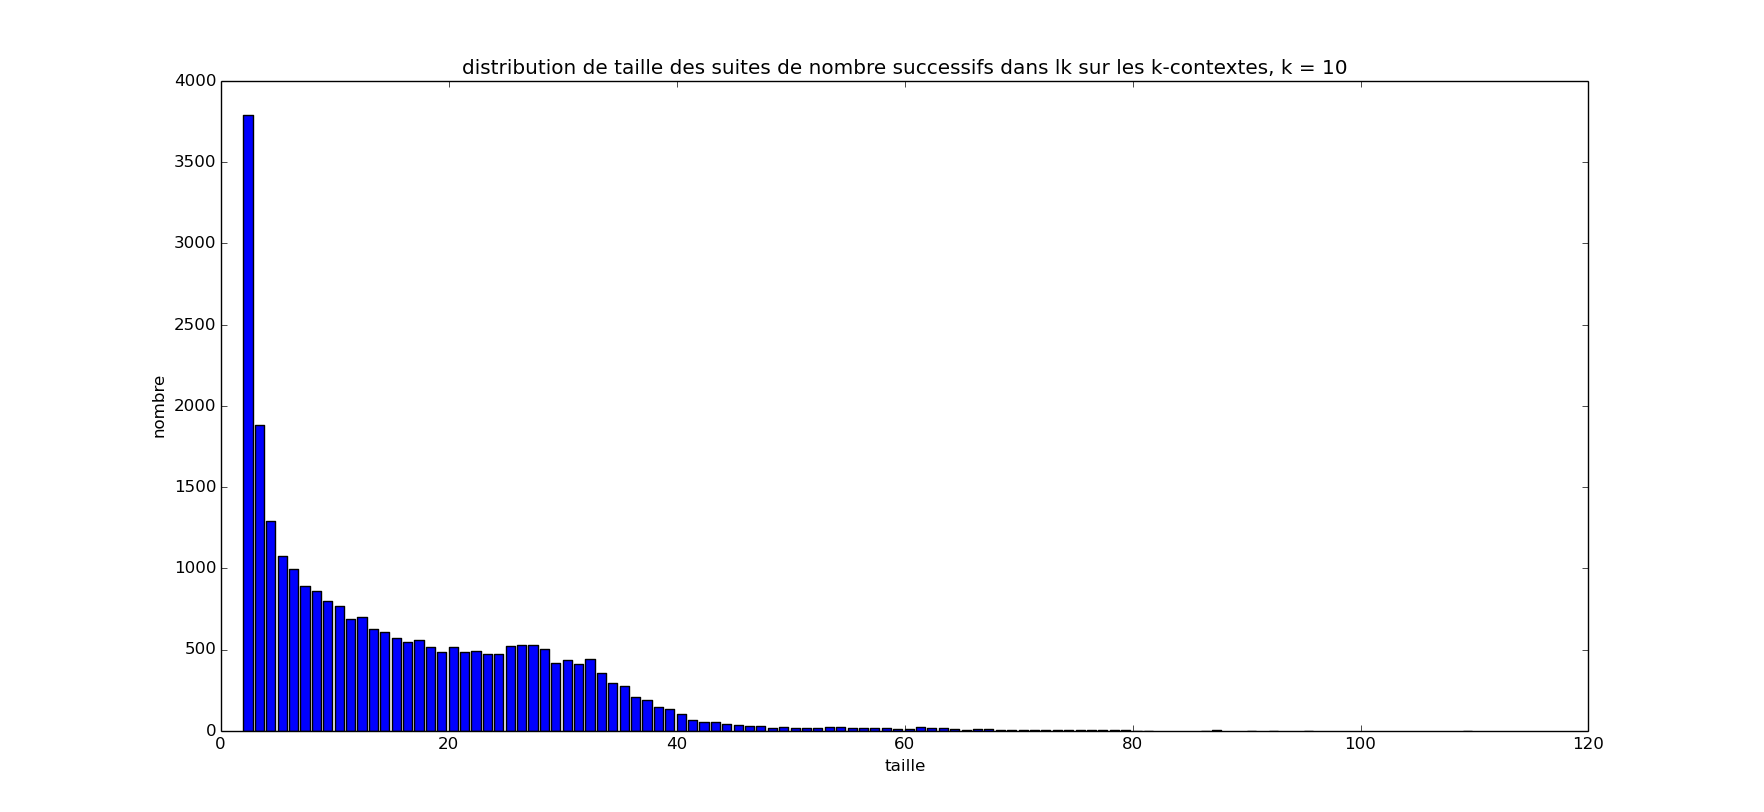
\includegraphics[scale = 0.3]{./images/suitesLFreads10K_k10.png}
    \caption{Distribution de taille des suites de nombres successifs dans LF() sur les k-contextes de la \kbwt\ triée pour $k = 10$ d'un ensemble Reads10K (ensemble de 500 reads de taille 70). On s'aperçoit qu'il y a plus de 7000 suites de nombres successifs supérieures à 20 dans les k-contextes.}
    \label{suitesLF}
\end{figure}

La deuxième approche consiste à regarder la différence entre la fonction LF() et $LF'(i) = C[i] + rank(\bwt[i], i)$, c'est-à-dire la fonction utilisée pour calculer LF() sur la \bwt. Avec cette méthode, il suffit pour retrouver LF() de calculer LF'() et lui ajouter la différence conservée.
%\rmq{S'agit-il de la différence entre LF($i$) et LF'$(i)$ ? Mais dans ce cas, en position i dans la \kbwt{} et dans la BWT nous n'avons pas forcément la même permutation circulaire. Il faut conserver le fait que LF nous amène à la permutation circulaire précédente.}



%
%Premières idées :
%	. chercher par blocs (-> seulement quand bloc assez grand)
%	. stocker permutations (-> infos ne peut pas se contenir elle meme ; décrire différentes idées stockage)

%Implémentation pour tester faisabilité         |  
%étude de la compression                        | -> dans Résultats ?
%calcul de l'entropie pour voir si correspond   | 
%compression avec compresseurs existants        |
%
%pour recherche, besoin de lf. pour lf besoin struc Petri -> lourd
%sur k-contextes, lf croissante -> stocker lf ? mieux
%
%lf lourde
%essais compression
%
%petits k-contextes qd \$ dans contexte -> enlever ces contextes ?
%non

\subsection{Résultats} 

%\textit{Cette section n'est donc pas finie, il manque des résultats dont une partie sur l'entropie, une sur les temps de calcul de recherche des motifs avec le stockage de LF(), et une sur les temps de calcul de la recherche de positions avec l'algorithme 1.}

Pour les résultats de cette section, nous nous sommes appuyés sur un jeu synthétique du génome lambda phage de 500 reads de taille 70, sans erreurs, appelé \textit{reads10K} ; ainsi qu'un jeu plus petit généré artificiellement et toujours sans erreurs, de 400 reads de taille 35, \textit{reads100}.

Nous avons étudié la compression de la \kbwt\ triée par rapport à la \kbwt\ présentée dans la thèse de Petri\up{\cite{petri}}. Comme attendu, on peut voir dans la figure \ref{tailleContextes} que les $k$-contextes de la \kbwt\ pour des reads sont grands et nombreux. La compression est donc meilleure (table \ref{struct}).

\begin{figure}[!ht]
    \center
    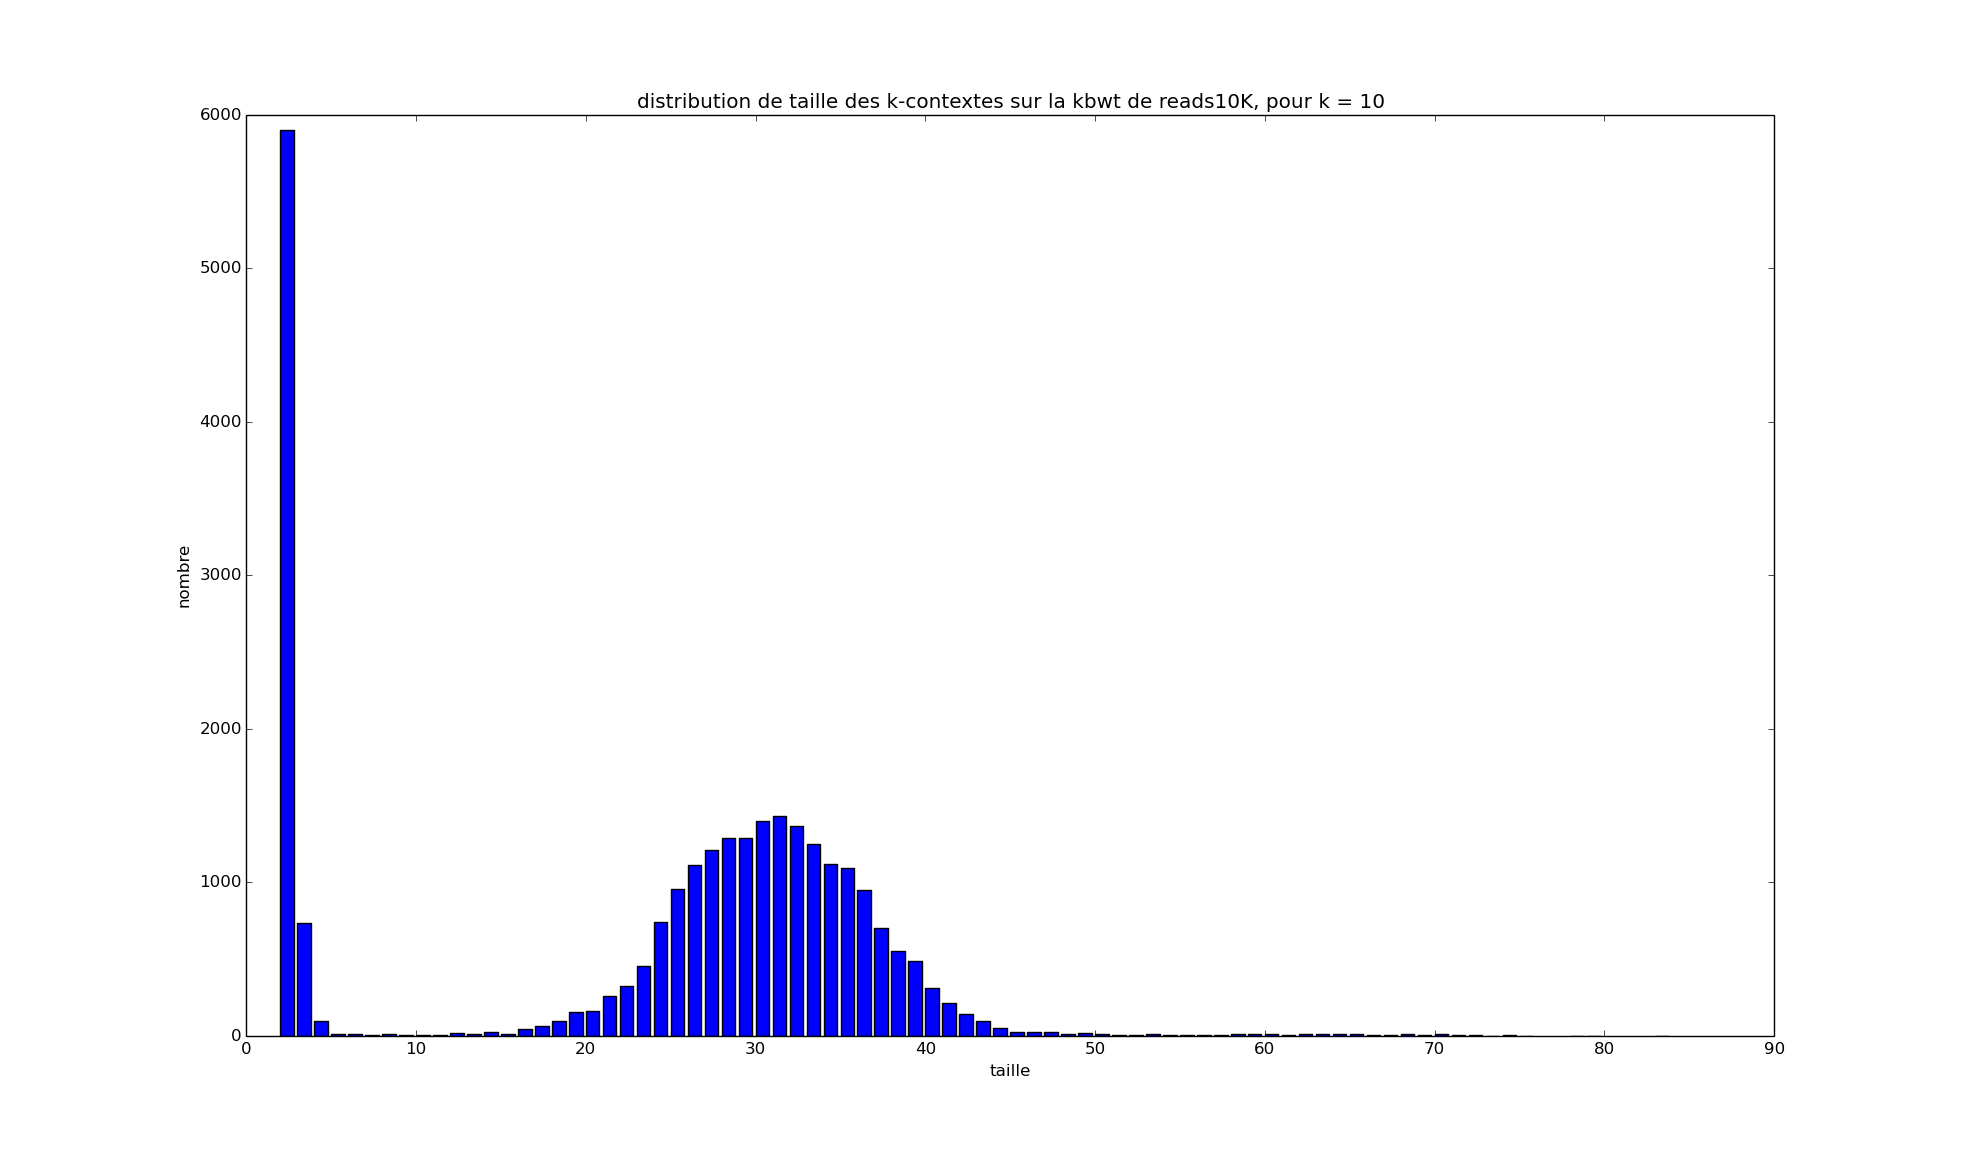
\includegraphics[scale=0.3]{./images/distribReads10K_k10.png}
    \caption{Distribution de taille des $k$-contextes sur la \kbwt\ triée de reads10K, pour $k = 10$. On peut voir que la \kbwt\ triée de cet ensemble comprend environ 15 000 $k$-contextes de taille entre 25 et 40. Les presque 6000 $k$-contextes de taille 2 correspondent aux $k$-contextes chevauchant deux reads.}
    \label{tailleContextes}
\end{figure}

\begin{table}
\centering
\begin{tabular}{|c||c|c|}
	\cline{2-3}
	\multicolumn{1}{c|}{} & reads10K & reads100\\ \cline{2-3} \hline
	fichier original & 51,8~ko & 706~octets\\ \hline
	\bwt & 48,3~ko & 941~octets\\ \hline
	\kbwt & 1,3~ko & 57,3~ko \\ \hline
	\kbwt\ triée & 51,4~ko & 935~octets \\ \hline
	\kbwt\ + $Dk$ & & \\ \hline
	\kbwt\ triée + $Dk$ + $Corr$ & & \\ \hline
\end{tabular}
\caption{Comparaison de la taille des différentes structures étudiées durant ce stage. Les \kbwt\ ont été calculées avec $k=10$. $Dk$ est le vecteur de bits contenant la délimitation des $k$-contextes, $Corr$ est le vecteur de bit introduit dans la section 2.2.1, correspondant au \textit{xor} entre le wavelet tree de la \kbwt\ et celui de la \kbwt\ triée. La compression a été effectuée avec le compresseur \textit{bzip2}.}
\label{struct}
\end{table}

De plus nous avons étudié l'espace pris par la fonction LF() suivant les deux approches décrites dans la section précédente (table \ref{resLF}). On s’aperçoit que la deuxième méthode, la comparaison des deux fonctions LF() et LF'() est légèrement plus compressible. Dans tous les cas, ces méthodes occupent beaucoup moins d'espace que les structures utilisées par Petri.

\begin{table}[h]
\centering
\begin{tabular}{|c|c||c|c|c|c|}
	\cline{3-6}
	\multicolumn{2}{c|}{} & \multicolumn{3}{c|}{reads10K} & reads100\\
	\cline{3-6}
\multicolumn{2}{c|}{}       
& $k=6$  & $k=10$  & $k=20$   & $k=10$ \\ \cline{3-6}\hline
\multicolumn{2}{|c||}{LF()}  
& 1,8~Mo & 1,9~Mo  & 1,2~Mo   & 21,5~ko \\ \hline
\multicolumn{2}{|c||}{LF'()}
& 1,2~Mo & 1,2~Mo  & 1,1~Mo   & 19,9~ko \\ \hline
\multicolumn{2}{|c||}{LF(i+1)-LF(i)} 
\color{red}& 1~Mo   & 1,3~Mo  & 142,2~ko & 5,1~ko  \\ \hline
\multicolumn{2}{|c||}{\color{red}LF()-LF'()}
& \color{red}1,2~Mo & \color{red}84,4~ko & \color{red}101,5~ko & \color{red}4,6~ko  \\ \hline
\multirow{4}{*}{Petri}
& $k-1$-\bwt &   9,5~ko    &   50,5~ko &       52,1~ko &     933~octets \\
& A          &   9,4~ko    &   55,8~ko &       88,9~ko &       1,5~ko \\
& S          &  204,8~ko   &   70,9~ko &       94,2~ko &       1,9~ko \\ \cline{2-6}
& Total &$\geq$~223,7~ko&$\geq$~177,2~ko&$\geq$~235,2~ko&$\geq$~4,3~ko \\ \hline
	
\end{tabular}
\caption{Comparaison de la taille prise par la fonction LF() selon différentes méthodes, pour la \kbwt\ triée de reads10K et reads100. Les dernières lignes du tableau montre l'espace utilisé par l'ensemble des structures utilisées par Petri pour calculer LF() sans la stocker. Seuls les vecteurs de bits ($D_k$ et $D_k-1$) n'ont pas été comptés. La compression a été effectuée avec le compresseur \textit{bzip2}.}
\label{resLF}
\end{table}


  \cleardoublepage
  \section*{Conclusion}
\addcontentsline{toc}{section}{Conclusion}

Pour conclure, ...

  \cleardoublepage
  \phantomsection\addcontentsline{toc}{section}{Références}
\begin{thebibliography}{ABC}	
    \bibitem[1]{bwt} Michael Burrows et D. J. Wheeler, \emph{A block-sorting lossless data compression algorithm}, 10th May 1994, Digital SRC Research Report 124.
    \bibitem[2]{petri} Matthias Petri, \emph{Scalable succinct indexing for large text collections}, July 2013.
    \bibitem[3]{sarray} Okanohara,D. and Sadakane,K. \emph{Practical entropy-compressed rank/select dictionary} , 2006, CoRR abs/cs/0610001.
%    \bibitem[2]{fmindex} Michael Burrows, D. J. Wheeler \emph{A block-sorting lossless data compression algorithm}, 10th May 1994, Digital SRC Research Report 124.
%    \bibitem[a]{tutoltx} tutoriel \LaTeX{} \emph{http://www.ukonline.be/programmation/latex/tutoriel/index.php}
%    \bibitem[b]{expltx} exemple de rapport de stage en \LaTeX{} \emph{http://blog.hikoweb.net/index.php?/post2011/11/06/Exemple-de-rapport-en-LaTeX}
\end{thebibliography}

\end{document}

